\subsection{Server}

\subsubsection{Architettura}
L'architettura del server è stata scelta tra due soluzioni, che sono state trattate più in dettaglio durante il Laboratorio di Reti di Calcolatori:

\begin{enumerate}
	\item multithread sincrona con I/O bloccante (\texttt{Sockets} di \texttt{Java IO});
	\item monothread sincrona con I/O non bloccante (\texttt{Selectors} di \texttt{Java NIO}).
\end{enumerate}

Le due soluzioni hanno pregi e difetti complementari, ma il trade-off principale è tra \textbf{velocità} e \textbf{scalabilità}. Ai fini di questo progetto didattico è stata ritenuta più importante la reattività, garantita (sotto carichi non eccessivi) dalla prima soluzione.
\medskip \\
Possiamo dividere il server in due livelli: \textbf{interfaccia} e \textbf{core}.

\begin{enumerate}
	\item A livello di interfaccia si trovano:
		\begin{enumerate}
			\item Il socket TCP del server
			\item L'API del servizio di registrazione utente
			\item Il servizio RMI di notifiche push.
		\end{enumerate}
	\item A livello core si trovano:
		\begin{enumerate}
			\item Il thread pool di client handlers
			\item I manager di utenti, documenti e indirizzi IP multicast.
		\end{enumerate}
\end{enumerate}

Per ogni client che si connette, il server riserva un thread, che si occuperà di gestire la connessione TCP per l'intero tempo di vita del client.

L'\textbf{automa a stati} del client di \texttt{TURING} è stato implementato con tre stati interni ad ogni client handler, perché non si può fare affidamento sulla buona scrittura del client.
\medskip \\
L'invio di messaggi \textbf{multicast} viene effettuato tramite un \textit{datagramChannel} che viene aperto quando c'è almeno un utente che sta modificando il documento, e chiuso quando nessuno lo sta più modificando.

\newpage

\begin{center}
	\begin{figure}[ht!]
		\makebox[\textwidth]{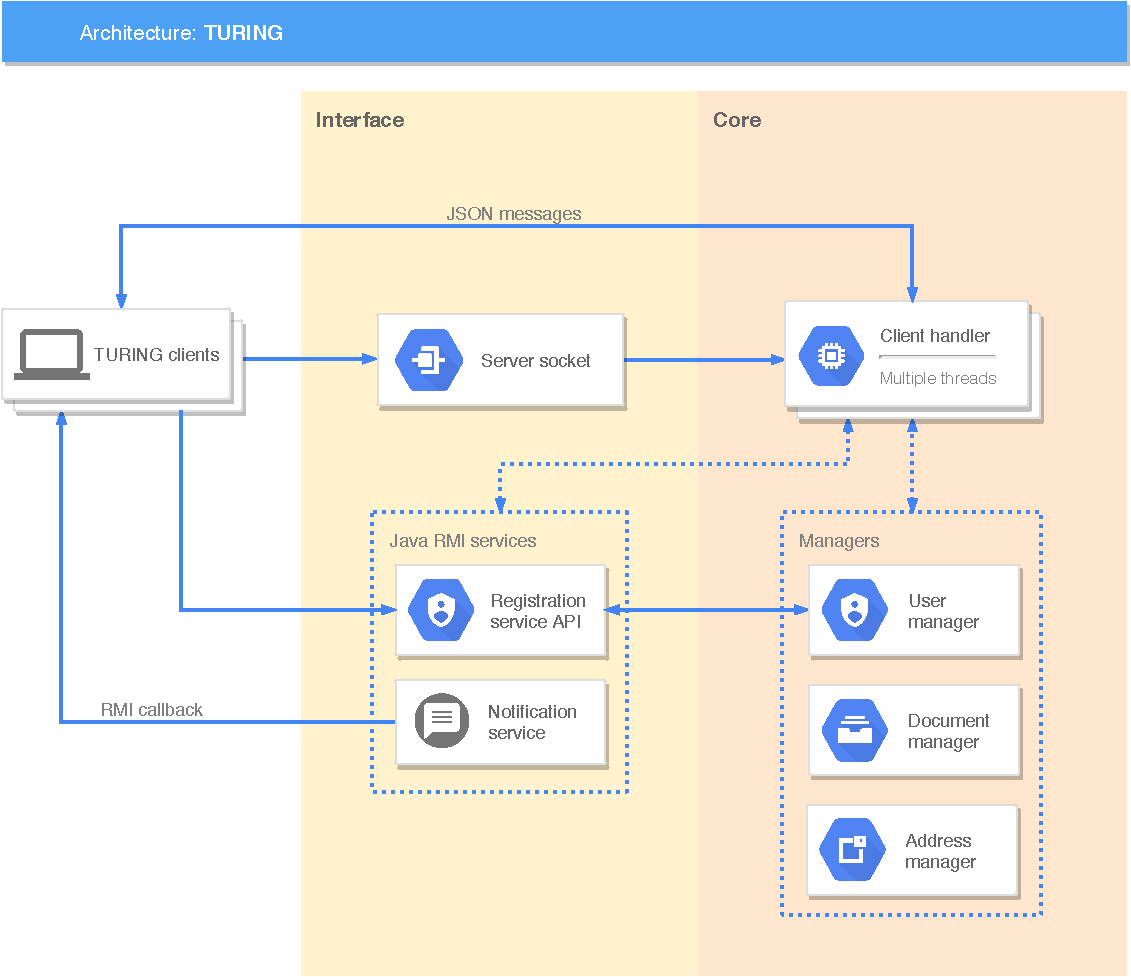
\includegraphics[width=0.75\paperwidth]{img/turing_architecture.pdf}}
		\caption{Architettura di \texttt{TURING} e interazioni tra le varie componenti.}
	\end{figure}
\end{center}

\subsubsection{Strutture dati}


\subsubsection{Protocollo di terminazione}
\sloppy
Quando il server viene terminato (a parte il caso eccezionale del segnale \texttt{SIGKILL}), viene avviata in un nuovo thread una routine di cleanup, dove:
\begin{itemize}
	\item viene chiuso il socket del server;
	\item viene attesa la terminazione dei thread del pool per un tempo massimo pari al doppio del tempo di risveglio dei socket verso i client; se dopo questo tempo qualche thread è ancora in esecuzione, viene terminato forzatamente;
	\item vengono cancellati tutti i file di testo salvati dagli utenti, in quanto il server non mantiene uno stato da caricare al riavvio.
\end{itemize}

\subsubsection{Organizzazione dei documenti}
I documenti vengono salvati come file di testo codificati nello standard \texttt{UTF-8}, rispettando la seguente gerarchia (utente $\rightarrow$ documento $\rightarrow$ sezione):

\medskip

\dirtree{%
	.1 data/.
	.2 Michele/.
	.3 relazione\_turing/.
	.4 1.
	.4 2.
	.4 3.
	.2 Dante Alighieri/.
	.3 Divina Commedia/.
	.4 1.
	.4 2.
	.4 \dots.
	.4 100.
	.3 De vulgari eloquentia/.
	.4 1.
	.4 2.
}
